\documentclass[conference]{IEEEtran}

\usepackage{cite}
\usepackage{amsmath,amssymb,amsfonts}
\usepackage{algorithm}
\usepackage{algorithmic}
\usepackage{graphicx}
\usepackage{booktabs}
\usepackage{textcomp}
\usepackage{flafter}

\renewcommand{\algorithmicrequire}{\textbf{Input:}}
\renewcommand{\algorithmicensure}{\textbf{Output:}}

\begin{document}

\title{Random Forests for Multiclass Network Intrusion Detection under Class Overlap}

\author{\IEEEauthorblockN{Student Number: 25913077}
\IEEEauthorblockA{\textit{Department of Computer Science} \\
\textit{Stellenbosch University}}}

\maketitle

\begin{abstract}
Ensemble learning combines predictions from multiple models to improve on a single model's predictions. The study investigated a random forest for multiclass network traffic classification on a modified version of the UNSW-NB15 dataset. The dataset contained 257,673 observations, 43 descriptive features, and 10 classes. A random forest was selected to investigate whether an ensemble of classification trees improves on the stronger of two classifiers developed in a preceding study, through bootstrap aggregation and random feature selection. Four questions were fixed before evaluation. The questions concerned the number of trees, the number of features considered per split, the complexity of the member trees, and class weighting. Control parameters were tuned sequentially using stratified five-fold cross-validation, with macro-averaged F1-score as the selection measure. The selected forest contained 75 fully grown, unweighted trees that considered 48 of approximately 75 encoded features at every split. The conventional square root rule gave eight features per split and produced a forest that was inferior to a single pruned tree. The selected model achieved a macro-averaged F1-score on a held-out generalisation set. The corresponding scores for a pruned classification tree and a nearest-neighbour classifier were 0.608 and 0.486. The improvement over the single tree was small. The McNemar test showed a statistically significant improvement in accuracy, and the macro-averaged F1-score improved consistently across all folds and seeds, without a formal significance test. An analysis of the dataset showed that 15.7\% of observations shared identical feature values with observations from a different class. Backdoor, denial of service, and analysis attacks were the most affected classes. Therefore, variance reduction through aggregation could not remove the dominant source of error.
\end{abstract}

\begin{IEEEkeywords}
ensemble learning, random forest, bagging, classification tree, network intrusion detection
\end{IEEEkeywords}

\section{Introduction}

Network intrusion detection involves assigning a class, such as normal traffic or a specific attack type, to an observed network flow. Moustafa and Slay introduced the UNSW-NB15 data set to facilitate the development of classifiers for network intrusion detection \cite{moustafa}. A prior study using a modified version of the UNSW-NB15 data set compared a $k$-nearest neighbour ($k$-NN) classifier with a classification tree, finding that the classification tree outperformed the $k$-NN classifier. However, both classifiers demonstrated limited effectiveness on the backdoor, analysis, and denial-of-service attack classes.

Ensemble learning aggregates the predictions of multiple models to improve classification performance. Breiman introduced bagging and random forests, two ensemble methods that average the outputs of classification trees generated from bootstrap samples \cite{breiman1996,breiman2001}. Unpruned classification trees typically exhibit low bias and high variance, and the prior study reported substantial overfitting on the same data set. Consequently, a tree-based ensemble was identified as a promising approach to enhance performance over a single classification tree.

This study pursued three objectives. First, an ensemble method was selected with a clear intention for the final comparative analysis. Second, the ensemble was tuned to address four predefined research questions. Third, the tuned ensemble was evaluated against the two classifiers from the prior study using identical data partitions and performance metrics.

Control parameters were tuned sequentially using stratified five-fold cross-validation on the development set and the same folds as the prior study, with macro-averaged F1-score serving as the selection criterion. The selected random forest and both baseline classifiers were subsequently evaluated on a held-out generalisation set.

The tuning process selected a random forest that considered 48 features per split, which exceeds the conventional square-root rule. The random forest achieved a marginal improvement in macro-averaged F1-score over both baseline classifiers. Further analysis of the data set attributed this small performance margin to the presence of observations from different classes sharing identical feature values.

The remainder of this report is structured as follows. Section~\ref{sec:background} provides background on the baseline classifiers and ensemble learning. Section~\ref{sec:method} outlines the rationale for the selected ensemble method, states the four research questions, and describes the implementation. Section~\ref{sec:procedure} details the empirical procedure. Section~\ref{sec:results} presents and discusses the research findings. Section~\ref{sec:conclusions} offers the conclusions. The source code developed for this study is available in a version-controlled repository.\footnote{\texttt{https://github.com/amoremoller/25913077-RW441-Assignment4.git}}

\section{Background}\label{sec:background}

Nearest neighbour classification and classification trees are described first, because both classifiers serve as baseline classifiers. Ensemble learning, bagging, and random forests are described thereafter.

\subsection{Nearest Neighbour Classification}

Cover and Hart introduced the nearest neighbour rule, where a query observation receives the class of the closest training observation \cite{cover}. The $k$-NN classifier generalises the rule to the $k$ closest training observations \cite{kelleher}. Training consists of storing the labelled training observations. Prediction is deferred until a query observation is presented.

For two feature vectors $\mathbf{x}_1$ and $\mathbf{x}_2$, each containing $N$ numerical descriptive features, the Minkowski distance is
\begin{equation}
d(\mathbf{x}_1,\mathbf{x}_2)=\left(\sum_{j=1}^{N}\left|x_{1j}-x_{2j}\right|^{w}\right)^{1/w},
\label{eq:minkowski}
\end{equation}
where $w$ denotes the order of the distance measure. The value $w=1$ gives the Manhattan distance, and the value $w=2$ gives the Euclidean distance \cite{kelleher}. Majority voting assigns equal influence to each of the $k$ neighbours. Distance-weighted voting gives closer neighbours greater influence on the predicted class \cite{kelleher}.

A small value of $k$ produces a classifier with low bias and high variance, and a large value of $k$ produces smoother decision boundaries \cite{kelleher}. Distances are accumulated over all descriptive features, so that the $k$-NN classifier is sensitive to differing feature ranges and high dimensionality \cite{kelleher}.

\subsection{Classification Trees}

A classification tree is a hierarchical collection of decision rules \cite{quinlan}. A non-terminal node tests a descriptive feature, and a leaf represents a predicted class. Tree induction recursively partitions the training set into increasingly homogeneous subsets. The impurity of a training set $D$ containing $M$ classes is measured using entropy as
\begin{equation}
H(D)=-\sum_{m=1}^{M}P(y_m)\log_2 P(y_m),
\label{eq:entropy}
\end{equation}
where $P(y_m)$ denotes the proportion of observations in $D$ that belong to class $y_m$. A candidate split on descriptive feature $x$ partitions $D$ into $O$ subsets. The information gain of the split is
\begin{equation}
G(x)=H(D)-\sum_{o=1}^{O}P_o H(D_o),
\label{eq:gain}
\end{equation}
where $D_o$ denotes the subset associated with outcome $o$, and $P_o$ denotes the proportion of observations assigned to $D_o$. The split with the largest information gain is selected at each node \cite{quinlan}.

A fully grown tree fits the training set closely and generalises poorly. Pre-pruning restricts tree growth through stopping criteria, such as a maximum depth or a minimum number of observations per leaf. Breiman \textit{et al.} proposed cost-complexity pruning, where subtrees are removed after induction when the reduction in training impurity per leaf is smaller than a threshold $\alpha$ \cite{cart}. A classification tree is unstable, because a small change to the training set frequently produces a different tree \cite{breiman1996}.

\subsection{Ensemble Learning}

An ensemble is a set of models with predictions that are combined into a single prediction. Dietterich noted that an ensemble is more accurate than the members only when the members are accurate and make different errors \cite{dietterich2000}. Identical members provide no benefit because they repeat the same errors. Diversity can be achieved by training members on different observations, training them on different descriptive features, or injecting randomness into the learning algorithm \cite{dietterich2000}.

The benefit of aggregation follows from decomposing prediction error into bias and variance. Hastie \textit{et al.} derived the variance of the average of $T$ identically distributed members \cite{hastie}. For members with variance $\sigma^2$ and pairwise correlation $\rho$, the variance of the average is
\begin{equation}
\rho\sigma^2+\frac{1-\rho}{T}\sigma^2.
\label{eq:variance}
\end{equation}
The second term of \eqref{eq:variance} vanishes as $T$ increases. The first term remains and is governed by the correlation between the members. The bias of the average equals the bias of a single member \cite{hastie}. Aggregation of independently trained members is therefore effective for members with low bias and high variance.

Boosting follows a different principle. Members are induced sequentially, and each member concentrates on the observations misclassified by the preceding members \cite{dietterich2000}. Dietterich observed that boosting places increasing weight on mislabelled observations and overfits when the training set contains noisy class labels \cite{dietterich2000}.

\subsection{Bagging}

Breiman proposed bootstrap aggregating, abbreviated to bagging \cite{breiman1996}. Each member is trained on a bootstrap sample, $|D|$ observations drawn from $D$ with replacement. The probability that a given observation appears in a bootstrap sample is $1-(1-1/|D|)^{|D|}$, approximately 0.632 for a large training set \cite{hastie}. Different bootstrap samples contain different observations and different duplicates. The members therefore differ.

The members' predictions are combined by majority voting or by averaging the class proportions they predict. Breiman showed that bagging improves unstable learners, such as classification trees, but not stable learners, such as nearest neighbour classifiers \cite{breiman1996}. Fully grown trees are preferred as members, because aggregation removes variance and leaves bias unchanged.

Observations excluded from a bootstrap sample are called out-of-bag observations. Each training observation is out-of-bag for approximately 36.8\% of the members. Breiman showed that predicting each training observation using only the members excluded from the bootstrap sample provides an estimate of generalisation performance without a separate validation set \cite{breiman2001}.

\subsection{Random Forests}

Ho proposed the random subspace method, in which each ensemble tree is induced from a random subset of descriptive features \cite{ho}. Breiman combined bagging with random feature selection in the random forest \cite{breiman2001}. Each tree of a random forest is induced from a bootstrap sample. At each node, the algorithm considers only $q$ randomly selected descriptive features for the split. The trees are fully grown and unpruned. Algorithm~\ref{alg:forest} summarises random forest induction. Bagging of classification trees is the special case where $q$ equals the number of descriptive features.

\begin{algorithm}[!t]
\caption{Random forest induction}
\label{alg:forest}
\begin{algorithmic}[1]
\REQUIRE Training set $D$, number of trees $T$, number of features per split $q$
\ENSURE Ensemble of $T$ classification trees
\FOR{each of the $T$ trees}
\STATE Draw a bootstrap sample of $|D|$ observations from $D$ with replacement
\STATE Create a root node containing the bootstrap sample
\WHILE{a node exists that is impure and has an admissible split}
\STATE Select $q$ descriptive features at random without replacement
\STATE Split the node on the selected feature and threshold with the largest reduction in impurity
\ENDWHILE
\STATE Add the unpruned tree to the ensemble
\ENDFOR
\STATE Return the ensemble
\end{algorithmic}
\end{algorithm}

Breiman showed that the generalisation error of a random forest converges as trees are added, so that additional trees do not cause overfitting \cite{breiman2001}. Breiman further showed that the generalisation error depends on two quantities, namely the strength of the individual trees and the correlation between the trees \cite{breiman2001}. A smaller $q$ reduces the correlation, consistent with \eqref{eq:variance}. A smaller $q$ also reduces the strength of individual trees because the most informative feature is often unavailable at a node. The square root of the number of descriptive features is the conventional value of $q$ for classification \cite{hastie}. Hastie \textit{et al.} noted that a random forest performs poorly with a small $q$ when only a small fraction of descriptive features is relevant \cite{hastie}.

The reduction in impurity contributed by each descriptive feature, summed over all trees, provides a measure of feature importance \cite{strobl}. Strobl \textit{et al.} showed that impurity-based importance is biased toward descriptive features with many distinct values \cite{strobl}.

\section{Methodology}\label{sec:method}

The methodology motivates the selection of the ensemble method, states the questions that directed the tuning, and describes the software implementation.

\subsection{Selection of the Ensemble Method}
A random forest was selected to investigate whether an ensemble of classification trees improves on the single-tree baseline through bootstrap aggregation and random feature selection. Random forest members are classification trees, the stronger baseline classifier from the preceding study. The single classification tree and the ensemble members share the same learning algorithm, impurity measure, and preprocessing. The two classifiers nevertheless differ in three respects. The forest aggregates trees induced from bootstrap samples, considers a random subset of features at every split, and uses fully grown member trees in place of a single pruned tree. Therefore, performance differences are attributable to the combination of these three differences, not aggregation alone.

The selection was further motivated by the preceding study, where an unpruned classification tree reached a mean training macro-averaged F1-score of 0.784 and a mean validation macro-averaged F1-score of 0.573. This gap indicated a low-bias, high-variance model, the case where bagging and random forests are effective \cite{breiman1996,breiman2001}.

Three alternatives were considered and rejected. Boosting was rejected because boosting is sensitive to noisy class labels \cite{dietterich2000}. The preceding study found persistent confusion between attack classes, indicating overlapping classes. An ensemble of $k$-NN classifiers was rejected because bagging does not improve stable learners \cite{breiman1996}. A stacked ensemble of the two baseline classifiers was rejected because the contribution of each member and of the combining model is difficult to separate.

\subsection{Research Questions}

Four questions were fixed before any ensemble was evaluated. Each question concerns a group of control parameters, and each question is accompanied by an expectation derived from the background.

\begin{enumerate}
\item \textit{Ensemble size.} The first question asks how many trees are required before performance stabilises. Performance was expected to increase with diminishing returns and without overfitting \cite{breiman2001}.
\item \textit{Features per split.} The second question asks how the value of $q$ affects the strength of the member trees, the diversity among the member trees, and the performance of the ensemble. A value of $q$ near the square root of the number of features was expected to provide the best balance between strength and diversity \cite{hastie}.
\item \textit{Tree complexity.} The third question asks whether the member trees require complexity control, as the single classification tree did. Fully grown member trees were expected to perform best, because averaging removes the variance of overfitted members \cite{breiman1996}.
\item \textit{Class weighting.} The fourth question asks whether class weighting improves the minority attack classes. Class weighting was expected to raise minority-class recall at the cost of precision, as observed for the single classification tree in the preceding study.
\end{enumerate}

\subsection{Software Implementation}
All classifiers were implemented in Python using the scikit-learn library \cite{sklearn}. SciPy provided the statistical distributions for the McNemar test, and Matplotlib produced the figures. All experiments were executed on a MacBook Air with an Apple M4 processor and 24~GB of memory, running macOS 26.3.1. Every available processor core was used for the induction of the forests and for the nearest neighbour searches.

Each classifier was implemented as a pipeline that combined the pre-processing operations with the classifier. Pre-processing operations with estimated quantities were therefore fitted only to the training observations of each cross-validation iteration.

The scikit-learn random forest implementation builds binary classification trees and draws bootstrap samples the same size as the training set. Member trees are combined by averaging the class proportions of the leaves reached by a query observation. The predicted class is the class with the largest mean proportion. The averaging rule is equivalent to majority voting when every leaf is pure. Ties are resolved in favour of the class with the lowest class index.

The trees of a random forest are induced independently. The first trees of a large forest therefore constitute a valid smaller forest. Validation performance at every ensemble size was obtained from a single forest per cross-validation iteration by accumulating the class proportions tree by tree.

\section{Empirical Procedure}\label{sec:procedure}

The empirical procedure specifies the data partitions, the pre-processing, the baseline classifiers, the tuning, the performance measures, and the analysis process.

\subsection{Dataset and Experimental Design}

The supplied dataset is a modified version of the UNSW-NB15 dataset \cite{moustafa}. The dataset contains 257,673 observations, 43 descriptive features, and a target feature with 10 classes. The classes comprise normal traffic and nine attack types. The attack types are reconnaissance, backdoor, denial of service (DoS), exploits, analysis, fuzzers, worms, shellcode, and generic attacks. The class distribution is highly skewed. Normal traffic accounts for 36.09\% of observations, and the Worms class accounts for 0.07\%.

The data set was partitioned once into a development set of 206,138 observations and a generalisation set of 51,535 observations using a stratified 80:20 split. Stratified five-fold cross-validation was applied within the development set. Kohavi showed that stratification reduces the variance of cross-validation estimates \cite{kohavi}. Stratification also ensured that each validation fold retained observations of the Worms class.

A random seed of 42 determined the data partition, the cross-validation folds, and the random number stream of every tree-based classifier. This seed matched the preceding study. The development set, generalisation set, and folds were therefore identical to the preceding study's partitions. The same partitions were used for all classifiers and for all ensemble configurations. No classifier used the generalisation set for control parameter tuning. A single partition into folds was used, and the cross-validation was not repeated with different partitions.

\subsection{Data Preprocessing}

Four descriptive features were removed for all classifiers, consistent with the preceding study. The feature \texttt{id} is a unique identifier without predictive information. The features \texttt{sloss} and \texttt{dloss} are almost perfectly correlated with \texttt{sbytes} and \texttt{dbytes}. The feature \texttt{is\_ftp\_login} contains invalid values and duplicates the information of \texttt{ct\_ftp\_cmd}. The remaining 39 descriptive features comprise 35 numerical features, one binary feature, and the three nominal features \texttt{proto}, \texttt{state}, and \texttt{service}.

Table~\ref{tab:preprocessing} summarises the transformations applied to each feature group. The tree-based classifiers used the classification-tree preprocessing from the preceding study without change. Identical preprocessing ensured that differences between the single tree and the ensemble were not due to data representation.

\begin{table*}[!t]
\caption{Transformations applied to the descriptive feature groups}
\label{tab:preprocessing}
\centering
\begin{tabular}{@{}lll@{}}
\toprule
Feature group & Classification tree and random forest & Nearest neighbour classifier \\
\midrule
Numerical & Passed through unchanged & Rescaled to $[0,1]$ using minimum-maximum scaling \\
\texttt{proto} & One-hot encoded with infrequent categories grouped & One-hot encoded with infrequent categories grouped \\
\texttt{state}, \texttt{service} & Missing \texttt{service} values represented by an explicit category, & Missing \texttt{service} values imputed using the mode, with a \\
 & followed by one-hot encoding & missingness indicator, followed by one-hot encoding \\
Binary & Passed through unchanged & Passed through unchanged \\
\bottomrule
\end{tabular}
\end{table*}

Numerical features were not scaled for the tree-based classifiers, because a split depends only on the ordering of the feature values. Feature-based outliers and the remaining correlated features were retained for the same reason, consistent with the preceding study.

The feature \texttt{service} was missing for 54.8\% of the observations. Missing values were represented by an explicit category, so that a tree is able to split on the absence of a service value. Nominal features were one-hot encoded, because the scikit-learn implementation requires numerical input. Categories of \texttt{proto} that occurred in fewer than 0.08\% of the training observations were grouped into a single category. The encoded data contained 75 features when fitted on the complete development set. Forty of the 75 encoded features were binary indicator features.

No resampling was applied, because the preceding study found that resampling did not improve macro-averaged F1-score. Class imbalance was instead addressed through class weighting.

\subsection{Baseline Classifiers}

The two baseline classifiers used the final configurations of the preceding study. The $k$-NN classifier used $k=7$, distance-weighted voting, and the Manhattan distance. The classification tree used the entropy impurity measure, a maximum depth of 30, a minimum of three observations per leaf, and cost-complexity pruning with $\alpha=4.64\times10^{-5}$.

The control parameters of the baseline classifiers were selected in the preceding study by cross-validation on the same development set and the same folds. The control parameters were therefore not tuned again. The baseline classifiers were evaluated again on the present partitions to confirm that the implementation reproduced the results of the preceding study.

\subsection{Control Parameter Tuning}

The tuning process began with an initial forest constructed according to the conventional random forest methodology. This initial forest employed the entropy impurity measure, fully grown unpruned trees, uniform class weights, and the square root rule for $q$, resulting in eight features per split. The entropy impurity measure was fixed to ensure consistency with the single classification tree.

The number of features considered at each split was set to 4, 8, 16, 32, 48, or all available features. The minimum number of observations required per leaf was set to 1, 3, 5, 10, or 25, while the maximum tree depth was set to 10, 20, 30, or left unrestricted. Class weighting was either omitted, balanced, or balanced per bootstrap sample. Tuning was performed sequentially, with each experiment beginning from the configuration selected in the previous experiment and varying only one control parameter. The configuration yielding the highest mean validation macro-averaged F1-score was retained. Experiments involving features per split, tree complexity, and class weighting utilized ensembles of 100 trees. The appropriateness of using 100 trees was confirmed on the initial forest prior to tuning.

Tree complexity was investigated by varying a single control parameter at a time. An additional configuration applied the complete set of pruned baseline tree settings to each member tree. Balanced class weighting assigned each class a weight inversely proportional to its frequency, calculated either once or separately for each bootstrap sample.

Ensemble size was evaluated in two stages, using forests of up to 300 trees assessed at 16 different sizes ranging from one to 300 trees. The first evaluation utilized the initial forest configuration. The second evaluation employed the configuration selected after the three tuning experiments to determine the final ensemble size. The final ensemble size was defined as the smallest number of trees for which the mean validation macro-averaged F1-score was within 0.001 of the highest mean score observed across all sizes.

\subsection{Performance Measures}

Five performance measures were computed for every classifier. The measures were accuracy, balanced accuracy, macro-averaged precision, macro-averaged recall, and macro-averaged F1-score. Let $c_m$ denote the number of evaluated observations of class $y_m$ that are classified correctly. Let $u_m$ denote the number of evaluated observations predicted as class $y_m$, and let $v_m$ denote the number of evaluated observations with actual class $y_m$. The precision, recall, and F1-score of class $y_m$ are
\begin{equation}
p_m=\frac{c_m}{u_m},\qquad r_m=\frac{c_m}{v_m},\qquad f_m=\frac{2p_mr_m}{p_m+r_m},
\label{eq:measures}
\end{equation}
respectively. The macro-averaged measures are the unweighted means of $p_m$, $r_m$, and $f_m$ over the $M$ classes. Balanced accuracy equals macro-averaged recall for a multiclass problem. Accuracy is the proportion of evaluated observations that are classified correctly.

Macro-averaged F1-score was the selection measure, in agreement with the preceding study. Accuracy is dominated by the frequent classes. A classifier that assigns every observation to the Normal class achieves an accuracy of 36.09\% with zero recall for every attack class. Macro-averaged F1-score assigns equal weight to every class and combines precision and recall.

Every measure was computed separately on each validation fold. Results are reported as the mean and the sample standard deviation over the five folds.

\subsection{Analysis Process}
For each ensemble configuration, three additional quantities were recorded. The strength of the member trees was quantified as the mean validation macro-averaged F1-score of the individual trees. Diversity among the member trees was assessed as the mean pairwise disagreement between the first 20 trees, where disagreement is defined as the proportion of validation observations for which the two trees predict different classes. The difference between the training and validation macro-averaged F1-score of the ensemble was used as a measure of overfitting.

The final forest and both baseline classifiers were trained on the complete development set and evaluated once on the generalisation set. Per-class F1-scores and confusion matrices were analyzed to identify which classes contributed to differences between the classifiers.

Three analyses were conducted to support the final comparison. First, the out-of-bag estimate of the final forest was compared with both the cross-validation estimate and the generalisation performance. Second, the final forest was trained an additional five times using seeds 43 to 47 to assess the dependence of generalisation performance on the random number stream. Third, the McNemar test with continuity correction was applied to the paired predictions on the generalisation set \cite{mcnemar}. Dietterich recommended the McNemar test for comparing two classifiers on a single test set \cite{dietterich1998}. A significance level of 0.05 was used. The McNemar test evaluates the accuracy of two classifiers but does not address macro-averaged F1-score.

An additional analysis was conducted after the tuning results were obtained. This analysis identified observations whose feature values matched those of an observation from a different class, referred to as observations in conflict. No classifier can correctly classify all observations in conflict. Assigning the most frequent class to each distinct feature vector provided in-sample reference values for accuracy and per-class F1-scores. This analysis used the complete dataset and was not employed for model selection.

\section{Research Results}\label{sec:results}

The research results are presented in the order of the empirical procedure, and each subsection discusses the observations with reference to the expectations stated in Section~\ref{sec:method}.

\subsection{Baseline Classifiers}
The classification tree achieved a mean macro-averaged validation F1-score of 0.5918 (SD = 0.0117). The $k$-NN classifier achieved a macro-averaged F1-score of 0.4845, with a standard deviation of 0.0062. Both means matched those reported in the preceding study. The implementation therefore reproduced the baseline classifiers. The standard deviations differed slightly from the preceding study because it reported the population standard deviation. The pruned tree had a mean of 1,705 leaves and a mean training macro-averaged F1-score of 0.6508.

\subsection{Ensemble Size}

Fig.~\ref{fig:size} shows the mean validation macro-averaged F1-score against the number of trees. The shaded bands indicate one standard deviation over the five folds. The horizontal line indicates the single classification tree.

\begin{figure}[!t]
\centering
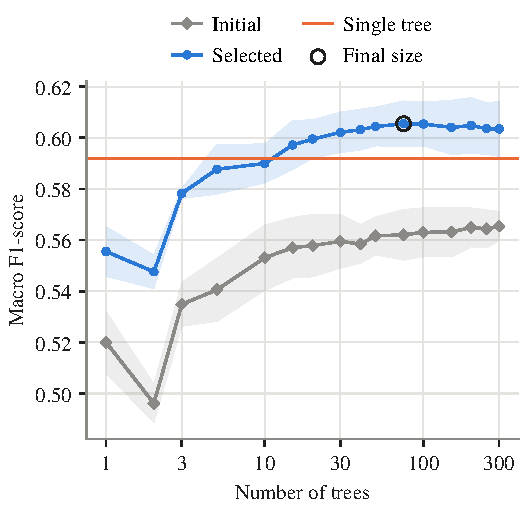
\includegraphics[width=\columnwidth]{figures/fig_ensemble_size.pdf}
\caption{Validation macro-averaged F1-score against ensemble size}
\label{fig:size}
\end{figure}

The initial forest's performance increased from 0.5200 with a single tree to 0.5630 with 100 trees. Adding 200 additional trees resulted in only a marginal improvement of 0.0024. Consequently, ensembles of 100 trees were deemed sufficient for the tuning experiments. At all sizes, the initial forest underperformed compared to the single classification tree. The conventional random forest was thus inferior to a single pruned tree on the selection measure. At 300 trees, the initial forest achieved an accuracy of 0.8273, while the single tree reached 0.8268. This deficit was specific to the macro-averaged measures.

The selected forest outperformed the single classification tree from 15 trees onward. The mean score peaked at 0.6055 with 75 trees and remained nearly constant at 0.6054 with 100 trees. According to the stated rule, 75 trees were selected. The mean score then declined slightly to 0.6035 at 300 trees. This decrease of 0.0020 was substantially smaller than the standard deviation of 0.0107 across folds. Thus, performance did not deteriorate significantly as more trees were added. This observation aligns with the expectation that increasing the number of trees does not lead to overfitting.

Both curves declined when increasing from one to two trees because two fully grown trees that disagree result in a tie, which is resolved in favor of the lowest class index.

\subsection{Number of Features per Split}

Table~\ref{tab:features} reports the results for the six values of $q$, and Fig.~\ref{fig:features} compares the ensemble with the mean member tree. The mean macro-averaged F1-score of the ensemble increased from 0.5399 with four features to 0.6054 with 48 features. The score decreased to 0.5999 when all features were considered. Consideration of 48 features was selected because the mean score was the highest. The scores for 32 features, 48 features, and all features differed by at most 0.0064, less than the standard deviation over the folds. The three values therefore formed a plateau, and the advantage of 48 features over the neighbouring values was not conclusive.

\begin{table}[!t]
\caption{Effect of the number of features considered per split}
\label{tab:features}
\centering
\setlength{\tabcolsep}{3.5pt}
\begin{tabular}{@{}lccccc@{}}
\toprule
 & Ensemble & & Member & & Worms \\
Features & macro F1 & Accuracy & macro F1 & Disagreement & F1 \\
\midrule
4 & $0.5399\pm0.0078$ & 0.8234 & 0.4951 & 0.1890 & 0.0937 \\
8 & $0.5630\pm0.0096$ & 0.8269 & 0.5129 & 0.1803 & 0.2477 \\
16 & $0.5842\pm0.0119$ & 0.8294 & 0.5332 & 0.1726 & 0.4041 \\
32 & $0.5990\pm0.0086$ & 0.8311 & 0.5498 & 0.1679 & 0.5074 \\
48 & $0.6054\pm0.0086$ & 0.8315 & 0.5548 & 0.1654 & 0.5607 \\
All & $0.5999\pm0.0099$ & 0.8302 & 0.5570 & 0.1629 & 0.5300 \\
\bottomrule
\end{tabular}
\end{table}

\begin{figure}[!t]
\centering
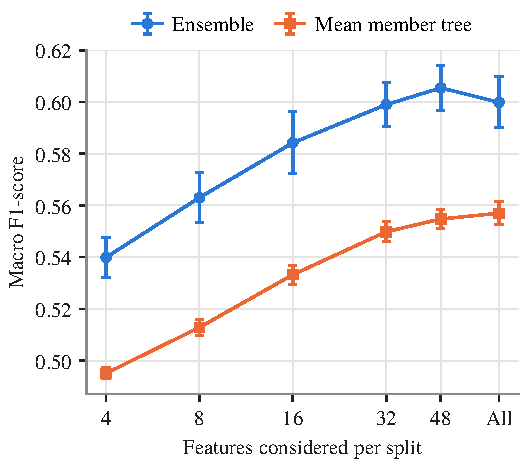
\includegraphics[width=\columnwidth]{figures/fig_max_features.pdf}
\caption{Validation macro-averaged F1-score of the ensemble and of the mean member tree against the number of features considered per split}
\label{fig:features}
\end{figure}

The observed results contradicted the expectation that the square root rule yields the optimal balance. Breiman accounted for this outcome using two metrics: strength and correlation \cite{breiman2001}. Increasing the number of features from 4 to 48 enhanced the strength of the member trees from 0.4951 to 0.5548, while the same increase reduced disagreement between member trees only from 0.1890 to 0.1654. Bootstrap sampling alone contributed most of the diversity. Across the range from four to 48 features, the increase in strength outweighed the reduction in diversity. Including all features further increased strength by 0.0022 and reduced disagreement by 0.0025, although the ensemble score decreased concurrently. This trade-off between strength and diversity resulted in an optimum at a high value of $q$, consistent with Breiman's theory.

The reduction in strength at small $q$ values aligned with the structure of the encoded data. The three most influential features in the final forest were \texttt{sbytes}, \texttt{service}, and \texttt{sttl}, with impurity-based importances of 0.214, 0.176, and 0.128, respectively. Collectively, these features accounted for 51.9\% of the total impurity reduction. More than half of the encoded features were binary indicators with limited individual informativeness. When a node considers eight random features, it often lacks access to a highly informative feature. This scenario matches the case described by Hastie \textit{et al.}, in which few features are relevant \cite{hastie}. Impurity-based importance tends to favor features with numerous distinct values \cite{strobl}. Consequently, the feature ranking was interpreted with caution.

The impact of $q$ was most pronounced in the rarest class. The F1-score for the Worms class increased from 0.0937 with four features to 0.5607 with 48 features. As a result, the Worms class contributed 0.0467 of the total increase of 0.0655 in macro-averaged F1-score. Accuracy varied by less than 0.009 across the six values and reached its highest value with 48 features. Thus, the selection of 48 features was not dependent on the specific selection metric.

\subsection{Tree Complexity}

Table~\ref{tab:complexity} reports the results of the tree complexity experiment. The column headed Gap reports the difference between the training and the validation macro-averaged F1-score.

\begin{table*}[!t]
\caption{Effect of complexity control applied to the member trees}
\label{tab:complexity}
\centering
\begin{tabular}{@{}lccccccc@{}}
\toprule
 & Ensemble & & Macro & & Member & & Leaves \\
Configuration & macro F1 & Accuracy & precision & Gap & macro F1 & Disagreement & per tree \\
\midrule
Fully grown & $0.6054\pm0.0086$ & 0.8315 & 0.7123 & 0.1754 & 0.5548 & 0.1654 & 8,856 \\
At least 3 observations per leaf & $0.6035\pm0.0104$ & 0.8312 & 0.7186 & 0.1362 & 0.5517 & 0.1678 & 6,627 \\
At least 5 observations per leaf & $0.5960\pm0.0123$ & 0.8300 & 0.7412 & 0.1013 & 0.5522 & 0.1642 & 5,158 \\
At least 10 observations per leaf & $0.5861\pm0.0135$ & 0.8291 & 0.7587 & 0.0606 & 0.5548 & 0.1543 & 3,065 \\
At least 25 observations per leaf & $0.5628\pm0.0038$ & 0.8257 & 0.7366 & 0.0331 & 0.5449 & 0.1339 & 1,418 \\
Maximum depth of 10 & $0.5087\pm0.0127$ & 0.8134 & 0.8027 & 0.0079 & 0.4901 & 0.0793 & 283 \\
Maximum depth of 20 & $0.5940\pm0.0097$ & 0.8318 & 0.7237 & 0.1485 & 0.5530 & 0.1417 & 4,949 \\
Maximum depth of 30 & $0.6034\pm0.0102$ & 0.8318 & 0.7105 & 0.1759 & 0.5548 & 0.1639 & 8,148 \\
Settings of the pruned baseline tree & $0.5975\pm0.0120$ & 0.8336 & 0.7680 & 0.0921 & 0.5621 & 0.1477 & 2,616 \\
\bottomrule
\end{tabular}
\end{table*}

Fully grown trees achieved the highest mean macro-averaged F1-score. These trees also exhibited one of the largest discrepancies between training and validation performance. Removing restrictions did not improve the validation score. This observation was consistent with prior expectations. Ensembles that overfit the training set more strongly demonstrated improved generalisation, as averaging reduced the variance among overfitted members.

Mild restrictions did not produce a significant effect, whereas strong restrictions were detrimental. Strong restrictions further reduced diversity among ensemble members. The disagreement metric decreased to 0.0793 at a maximum depth of ten, indicating that shallow trees generated largely identical predictions.

The pruned baseline tree settings demonstrated the trade-off between predictive strength and diversity. Pruned member trees achieved the highest individual mean score of 0.5621 but exhibited reduced diversity, with a disagreement value of 0.1477. The resulting ensemble attained the highest accuracy among all configurations, yet a lower macro-averaged F1-score compared to fully grown trees. Thus, pruning was advantageous for individual trees but unnecessary for the ensemble.

\subsection{Class Weighting}

Table~\ref{tab:weights} reports the results of the class weighting experiment. Balanced class weighting raised balanced accuracy and lowered macro-averaged precision and macro-averaged F1-score. Uniform class weights were therefore retained. The observation agreed with the expectation and repeated the behaviour of the single classification tree in the preceding study.

\begin{table}[!t]
\caption{Effect of class weighting}
\label{tab:weights}
\centering
\setlength{\tabcolsep}{3.5pt}
\begin{tabular}{@{}lcccc@{}}
\toprule
 & & Balanced & Macro & \\
Class weighting & Accuracy & accuracy & precision & Macro F1 \\
\midrule
None & 0.8315 & 0.5834 & 0.7123 & $0.6054\pm0.0086$ \\
Balanced & 0.7755 & 0.6199 & 0.5897 & $0.5861\pm0.0040$ \\
Per bootstrap sample & 0.7999 & 0.5935 & 0.6171 & $0.5935\pm0.0094$ \\
\bottomrule
\end{tabular}
\end{table}

The per-class results explained the trade-off. Balanced weighting increased the recall of the Backdoor class from 0.101 to 0.208 and the recall of the Analysis class from 0.106 to 0.175. The F1-scores of the same classes decreased from 0.173 to 0.049 and from 0.183 to 0.069. The recall of the Exploits class decreased from 0.820 to 0.565. Weighting therefore moved predictions from the Exploits class to the minority classes without an improvement in the separation of the classes. Class weighting changes the cost of an error and does not add information that distinguishes the classes.

\subsection{Comparison of the Classifiers}

The final random forest consisted of 75 fully grown classification trees induced from bootstrap samples, with 48 features considered at every split, the entropy impurity measure, and uniform class weights. Table~\ref{tab:comparison} reports the performance of the three classifiers under cross-validation and on the generalisation set.

\begin{table*}[!t]
\caption{Performance of the final classifiers under cross-validation and on the generalisation set}
\label{tab:comparison}
\centering
\begin{tabular}{@{}lcccccccc@{}}
\toprule
 & \multicolumn{4}{c}{Cross-validation} & \multicolumn{4}{c}{Generalisation set} \\
\cmidrule(lr){2-5}\cmidrule(l){6-9}
 & & Balanced & Macro & & & Balanced & Macro & \\
Classifier & Accuracy & accuracy & precision & Macro F1 & Accuracy & accuracy & precision & Macro F1 \\
\midrule
Nearest neighbour & $0.7850\pm0.0015$ & $0.4633\pm0.0052$ & $0.5758\pm0.0156$ & $0.4845\pm0.0062$ & 0.7866 & 0.4633 & 0.5841 & 0.4858 \\
Classification tree & $0.8268\pm0.0015$ & $0.5736\pm0.0165$ & $0.7043\pm0.0132$ & $0.5918\pm0.0117$ & 0.8273 & 0.6024 & 0.7199 & 0.6080 \\
Random forest & $0.8312\pm0.0007$ & $0.5837\pm0.0132$ & $0.7108\pm0.0099$ & $0.6055\pm0.0089$ & 0.8315 & 0.6018 & 0.7321 & 0.6221 \\
\bottomrule
\end{tabular}
\end{table*}
The random forest achieved the highest values across all evaluation metrics under cross-validation. On the generalisation set, the classification tree's balanced accuracy was marginally higher, at 0.6024 compared to 0.6018 for the random forest. However, the random forest outperformed the classification tree by 0.014 in macro-averaged F1-score under both cross-validation and on the generalisation set. The random forest consistently led across all five folds, with a mean paired difference of 0.0137 and a standard deviation of 0.0066.

This improvement was not attributable to random seed selection. Six random forests trained with different seeds achieved macro-averaged F1-scores ranging from 0.6161 to 0.6230, all exceeding the classification tree's score of 0.6080.

The McNemar test revealed a significant difference in accuracy between the random forest and the classification tree. The random forest correctly classified 2,007 observations that the classification tree did not, while the classification tree was correct for 1,790 observations missed by the random forest. The test statistic was 12.29, corresponding to a probability below 0.001. The net advantage of 217 observations represented 0.42\% of the generalisation set. Thus, the difference in accuracy was statistically significant but of limited practical magnitude. The difference compared to the $k$-NN classifier was also significant, with a test statistic of 899.1.

The out-of-bag estimate of the macro-averaged F1-score was 0.6087, closely aligning with the cross-validation estimate of 0.6055, and required only a single forest induction. Both classifiers achieved higher scores on the generalisation set than under cross-validation. The final classifiers were trained on the complete development set, which was 25\% larger than the training set used in each cross-validation iteration.

The observed improvement was accompanied by increased computational cost. On the hardware described in Section~\ref{sec:method}, training the random forest required 15.9 seconds, compared to 2.5 seconds for the classification tree. The member trees of the random forest had a mean of 8,858 leaves, whereas the single pruned tree had 1,705 leaves. Consequently, the random forest also reduced interpretability.

Table~\ref{tab:classes} presents the F1-scores for each class on the generalisation set. The random forest achieved higher F1-scores than the classification tree in eight of ten classes, with the largest gains in the Analysis, DoS, and Fuzzers classes. The classification tree outperformed the random forest in the Exploits and Worms classes. However, the Worms class included only 35 generalisation observations, so the three-prediction difference does not reliably indicate a model weakness.

\begin{table}[!t]
\caption{F1-score for every class on the generalisation set, with the share of observations in conflict and the reference F1-score from the class overlap analysis}
\label{tab:classes}
\centering
\setlength{\tabcolsep}{3pt}
\begin{tabular}{@{}lrccccc@{}}
\toprule
 & & Nearest & & Random & In & Refer- \\
Class & Support & neighbour & Tree & forest & conflict & ence \\
\midrule
Normal & 18,600 & 0.903 & 0.923 & 0.934 & 1.0\% & 0.996 \\
Reconnaissance & 2,798 & 0.660 & 0.834 & 0.837 & 16.1\% & 0.914 \\
Backdoor & 466 & 0.054 & 0.156 & 0.179 & 84.9\% & 0.265 \\
DoS & 3,271 & 0.354 & 0.274 & 0.305 & 77.4\% & 0.539 \\
Exploits & 8,905 & 0.676 & 0.732 & 0.724 & 37.1\% & 0.812 \\
Analysis & 535 & 0.190 & 0.179 & 0.212 & 77.0\% & 0.375 \\
Fuzzers & 4,849 & 0.525 & 0.629 & 0.658 & 14.9\% & 0.924 \\
Worms & 35 & 0.163 & 0.718 & 0.714 & 8.6\% & 0.957 \\
Shellcode & 302 & 0.347 & 0.649 & 0.668 & 0.9\% & 0.996 \\
Generic & 11,774 & 0.985 & 0.986 & 0.989 & 0.6\% & 0.997 \\
\bottomrule
\end{tabular}
\end{table}

Fig.~\ref{fig:confusion} shows the confusion matrix of the random forest on the generalisation set, as percentages of the actual class. The dominant pattern of the preceding study persisted. The random forest assigned 68.7\% of the DoS observations, 58.4\% of the Backdoor observations, and 51.0\% of the Analysis observations to the Exploits class. The corresponding percentages for the classification tree were 75.0\%, 76.2\%, and 62.6\%. Aggregation therefore reduced the confusion with the Exploits class without removing the confusion. The random forest assigned 26.2\% of the Fuzzers observations to the Normal class, compared with 28.7\% for the classification tree.

\begin{figure}[!t]
\centering
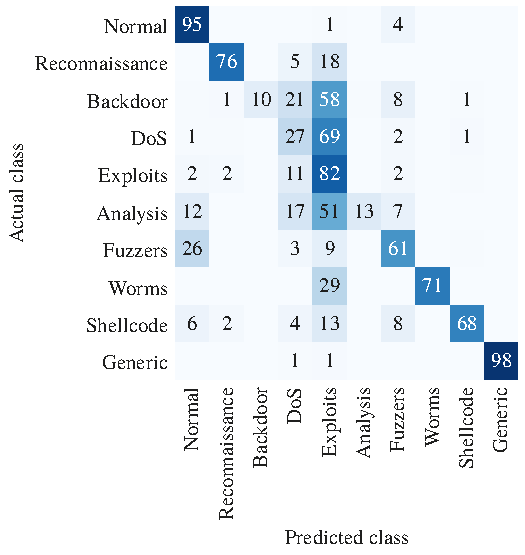
\includegraphics[width=\columnwidth]{figures/fig_confusion_forest.pdf}
\caption{Confusion matrix of the random forest on the generalisation set, as percentages of the actual class}
\label{fig:confusion}
\end{figure}

\subsection{Class Overlap}

The limited improvement achieved through aggregation prompted an analysis of class overlap. The dataset comprised 153,684 distinct feature vectors among 257,673 observations. Of these, 40,400 observations, representing 15.7\% of the dataset, were identified as conflicting.

The last two columns of Table~\ref{tab:classes} report the share of conflicting observations and the reference F1-score for each class. Conflicts were concentrated in four attack classes. The share was 84.9\% for the Backdoor class, 77.4\% for the DoS class, 77.0\% for the Analysis class, and 37.1\% for the Exploits class. The most conflicted class was the one all three classifiers assigned to Exploits. The Exploits class is the most frequent of the four classes. A classifier that minimises errors therefore assigns a contested feature vector to the Exploits class.

Assigning the most frequent class to each distinct feature vector resulted in an accuracy of 0.914 and a macro-averaged F1-score of 0.777. The reference F1-scores were 0.265 for Backdoor, 0.539 for DoS, and 0.375 for Analysis. In comparison, the random forest achieved F1-scores of 0.179, 0.305, and 0.212 for these classes, respectively. The substantial overlap among these three classes suggests that the available descriptive features alone cannot eliminate a significant portion of the classification error. These reference values reflect in-sample assignments rather than generalization estimates, so the analysis does not demonstrate that all observed errors are irreducible. The error component arising from identical feature vectors is not attributable to variance. Therefore, aggregating high-variance classifiers cannot eliminate this component. The same reasoning applies to class weighting, which also limits the potential benefit of alternative ensemble methods.

The analysis did not account for all observed weaknesses. For example, the Fuzzers class achieved a reference F1-score of 0.924, compared to 0.658 for the random forest. The confusion between the Fuzzers and Normal classes was therefore not attributable to identical feature vectors, indicating that further improvement for the Fuzzers class is possible.

Alternative circumstances could yield different results. Incorporating descriptive features that better distinguish attack classes would likely reduce conflict and improve attainable performance. The original UNSW-NB15 dataset includes address and port features that are absent from the supplied dataset \cite{moustafa}. A training set with less class overlap would also more clearly demonstrate the benefits of variance reduction.

Three limitations affect these results. First, tuning was performed sequentially, so interactions between control parameters were not assessed. Second, only a single partition into folds was used, making differences smaller than the standard deviation across folds, such as those between 32, 48, and all features, inconclusive. Third, the class overlap analysis was conducted after tuning and used the complete dataset, rendering the reference values optimistic.

\section{Conclusions}\label{sec:conclusions}
This study examined ensemble learning methods for multiclass network traffic classification using a modified UNSW-NB15 dataset. A random forest was employed to determine whether an ensemble of classification trees, constructed via bootstrap aggregation and random feature selection, outperforms a single classification tree. Control parameters were sequentially tuned using stratified five-fold cross-validation to address four predefined research questions. The optimized random forest was compared to both a classification tree and a $k$-nearest neighbour ($k$-NN) classifier from a previous study, utilizing identical data partitions.

Performance stabilized with ensembles of approximately 75 trees. The conventional square root rule for feature selection resulted in weak member trees and produced a forest that performed worse than a single pruned tree. Increasing the number of features considered at each split improved performance, reaching a plateau between 32 features and the full feature set. Complexity control for member trees was unnecessary, although pruning benefited the single tree. Applying class weighting increased balanced accuracy but reduced the macro-averaged F1-score.

The random forest achieved a macro-averaged F1-score of 0.622 on the generalization set, compared to 0.608 for the classification tree and 0.486 for the $k$-NN classifier. The improvement over the classification tree was consistent across all five folds and six random seeds. The McNemar test indicated that the accuracy improvement was statistically significant. However, no formal significance test was conducted for the macro-averaged F1-score.

The limited improvement is attributable to characteristics of the dataset. Specifically, 15.7\% of observations possessed feature values identical to those of observations from different classes. The backdoor, denial-of-service (DoS), and analysis attack classes were most affected by this overlap. Consequently, a substantial proportion of classification errors could not be resolved using the available descriptive features and thus persisted despite aggregation.

The findings demonstrate that a conventional random forest does not necessarily outperform a single pruned tree when only a few descriptive features contain most of the relevant information. Retaining strong member trees required a large number of features per split. Future research should investigate additional descriptive features that can better distinguish overlapping attack classes. Further examination of the confusion between the Fuzzers class and the Normal class is also warranted, as improvement remains possible in this area.

\appendices

\section{Symbols}

\begin{center}
\footnotesize
\begin{tabular}{@{}lp{0.72\columnwidth}@{}}
\toprule
Symbol & Definition \\
\midrule
$\alpha$ & cost-complexity pruning threshold \\
$c_m$ & number of evaluated observations of class $y_m$ classified correctly \\
$d$ & Minkowski distance function \\
$D$ & training set \\
$D_o$ & subset of $D$ associated with split outcome $o$ \\
$f_m$ & F1-score of class $y_m$ \\
$G$ & information gain function \\
$H$ & entropy function \\
$k$ & number of nearest neighbours \\
$M$ & number of classes \\
$N$ & number of descriptive features \\
$O$ & number of split outcomes \\
$p_m$ & precision of class $y_m$ \\
$P(y_m)$ & proportion of observations that belong to class $y_m$ \\
$P_o$ & proportion of observations assigned to $D_o$ \\
$q$ & number of features considered per split \\
$r_m$ & recall of class $y_m$ \\
$\rho$ & pairwise correlation between ensemble members \\
$\sigma^2$ & variance of an ensemble member \\
$T$ & number of ensemble members \\
$u_m$ & number of evaluated observations predicted as class $y_m$ \\
$v_m$ & number of evaluated observations with actual class $y_m$ \\
$w$ & order of the Minkowski distance \\
$x$ & descriptive feature \\
$\mathbf{x}$ & feature vector \\
$y_m$ & class $m$ \\
\bottomrule
\end{tabular}
\end{center}

\begin{thebibliography}{00}
\bibitem{breiman1996} L. Breiman, ``Bagging predictors,'' \textit{Machine Learning}, vol. 24, no. 2, pp. 123--140, 1996.
\bibitem{breiman2001} L. Breiman, ``Random forests,'' \textit{Machine Learning}, vol. 45, no. 1, pp. 5--32, 2001.
\bibitem{cart} L. Breiman, J. H. Friedman, R. A. Olshen, and C. J. Stone, \textit{Classification and Regression Trees}. Boca Raton, FL, USA: Chapman and Hall/CRC, 1984.
\bibitem{cover} T. Cover and P. Hart, ``Nearest neighbor pattern classification,'' \textit{IEEE Transactions on Information Theory}, vol. 13, no. 1, pp. 21--27, 1967.
\bibitem{dietterich1998} T. G. Dietterich, ``Approximate statistical tests for comparing supervised classification learning algorithms,'' \textit{Neural Computation}, vol. 10, no. 7, pp. 1895--1923, 1998.
\bibitem{dietterich2000} T. G. Dietterich, ``Ensemble methods in machine learning,'' in \textit{Proceedings of the First International Workshop on Multiple Classifier Systems}, ser. Lecture Notes in Computer Science, vol. 1857. Cagliari, Italy: Springer, 2000, pp. 1--15.
\bibitem{hastie} T. Hastie, R. Tibshirani, and J. Friedman, \textit{The Elements of Statistical Learning: Data Mining, Inference, and Prediction}, 2nd ed. New York, NY, USA: Springer, 2009.
\bibitem{ho} T. K. Ho, ``The random subspace method for constructing decision forests,'' \textit{IEEE Transactions on Pattern Analysis and Machine Intelligence}, vol. 20, no. 8, pp. 832--844, 1998.
\bibitem{kelleher} J. D. Kelleher, B. Mac Namee, and A. D'Arcy, \textit{Fundamentals of Machine Learning for Predictive Data Analytics: Algorithms, Worked Examples, and Case Studies}. Cambridge, MA, USA: MIT Press, 2020.
\bibitem{kohavi} R. Kohavi, ``A study of cross-validation and bootstrap for accuracy estimation and model selection,'' in \textit{Proceedings of the International Joint Conference on Artificial Intelligence}, Montreal, Canada, 1995, pp. 1137--1143.
\bibitem{mcnemar} Q. McNemar, ``Note on the sampling error of the difference between correlated proportions or percentages,'' \textit{Psychometrika}, vol. 12, no. 2, pp. 153--157, 1947.
\bibitem{moustafa} N. Moustafa and J. Slay, ``UNSW-NB15: A comprehensive data set for network intrusion detection systems,'' in \textit{Proceedings of the Military Communications and Information Systems Conference}, Canberra, Australia, 2015, pp. 1--6.
\bibitem{sklearn} F. Pedregosa \textit{et al.}, ``Scikit-learn: Machine learning in Python,'' \textit{Journal of Machine Learning Research}, vol. 12, pp. 2825--2830, 2011.
\bibitem{quinlan} J. R. Quinlan, \textit{C4.5: Programs for Machine Learning}. San Mateo, CA, USA: Morgan Kaufmann, 1993.
\bibitem{strobl} C. Strobl, A.-L. Boulesteix, A. Zeileis, and T. Hothorn, ``Bias in random forest variable importance measures: Illustrations, sources and a solution,'' \textit{BMC Bioinformatics}, vol. 8, art. no. 25, 2007.
\end{thebibliography}

\end{document}
